\chapter{Results and analysis}\label{chapter:res-analysis}

\section{SPM and distgen}\label{section:spmydistgen}
This section will discussed the different scenarios that will be used for the testing of distgen as observed process. For an overview of Distgen, please refer to section \ref{section:distgen}.
\subsection{SPM and distgen with two threads}\label{subsection:res-spmydistgen-2t}

\subsubsection{Scenarios under consideration}\label{subsection:res-scenarios-2t-scens}

\begin{figure}[th]
	\centering
		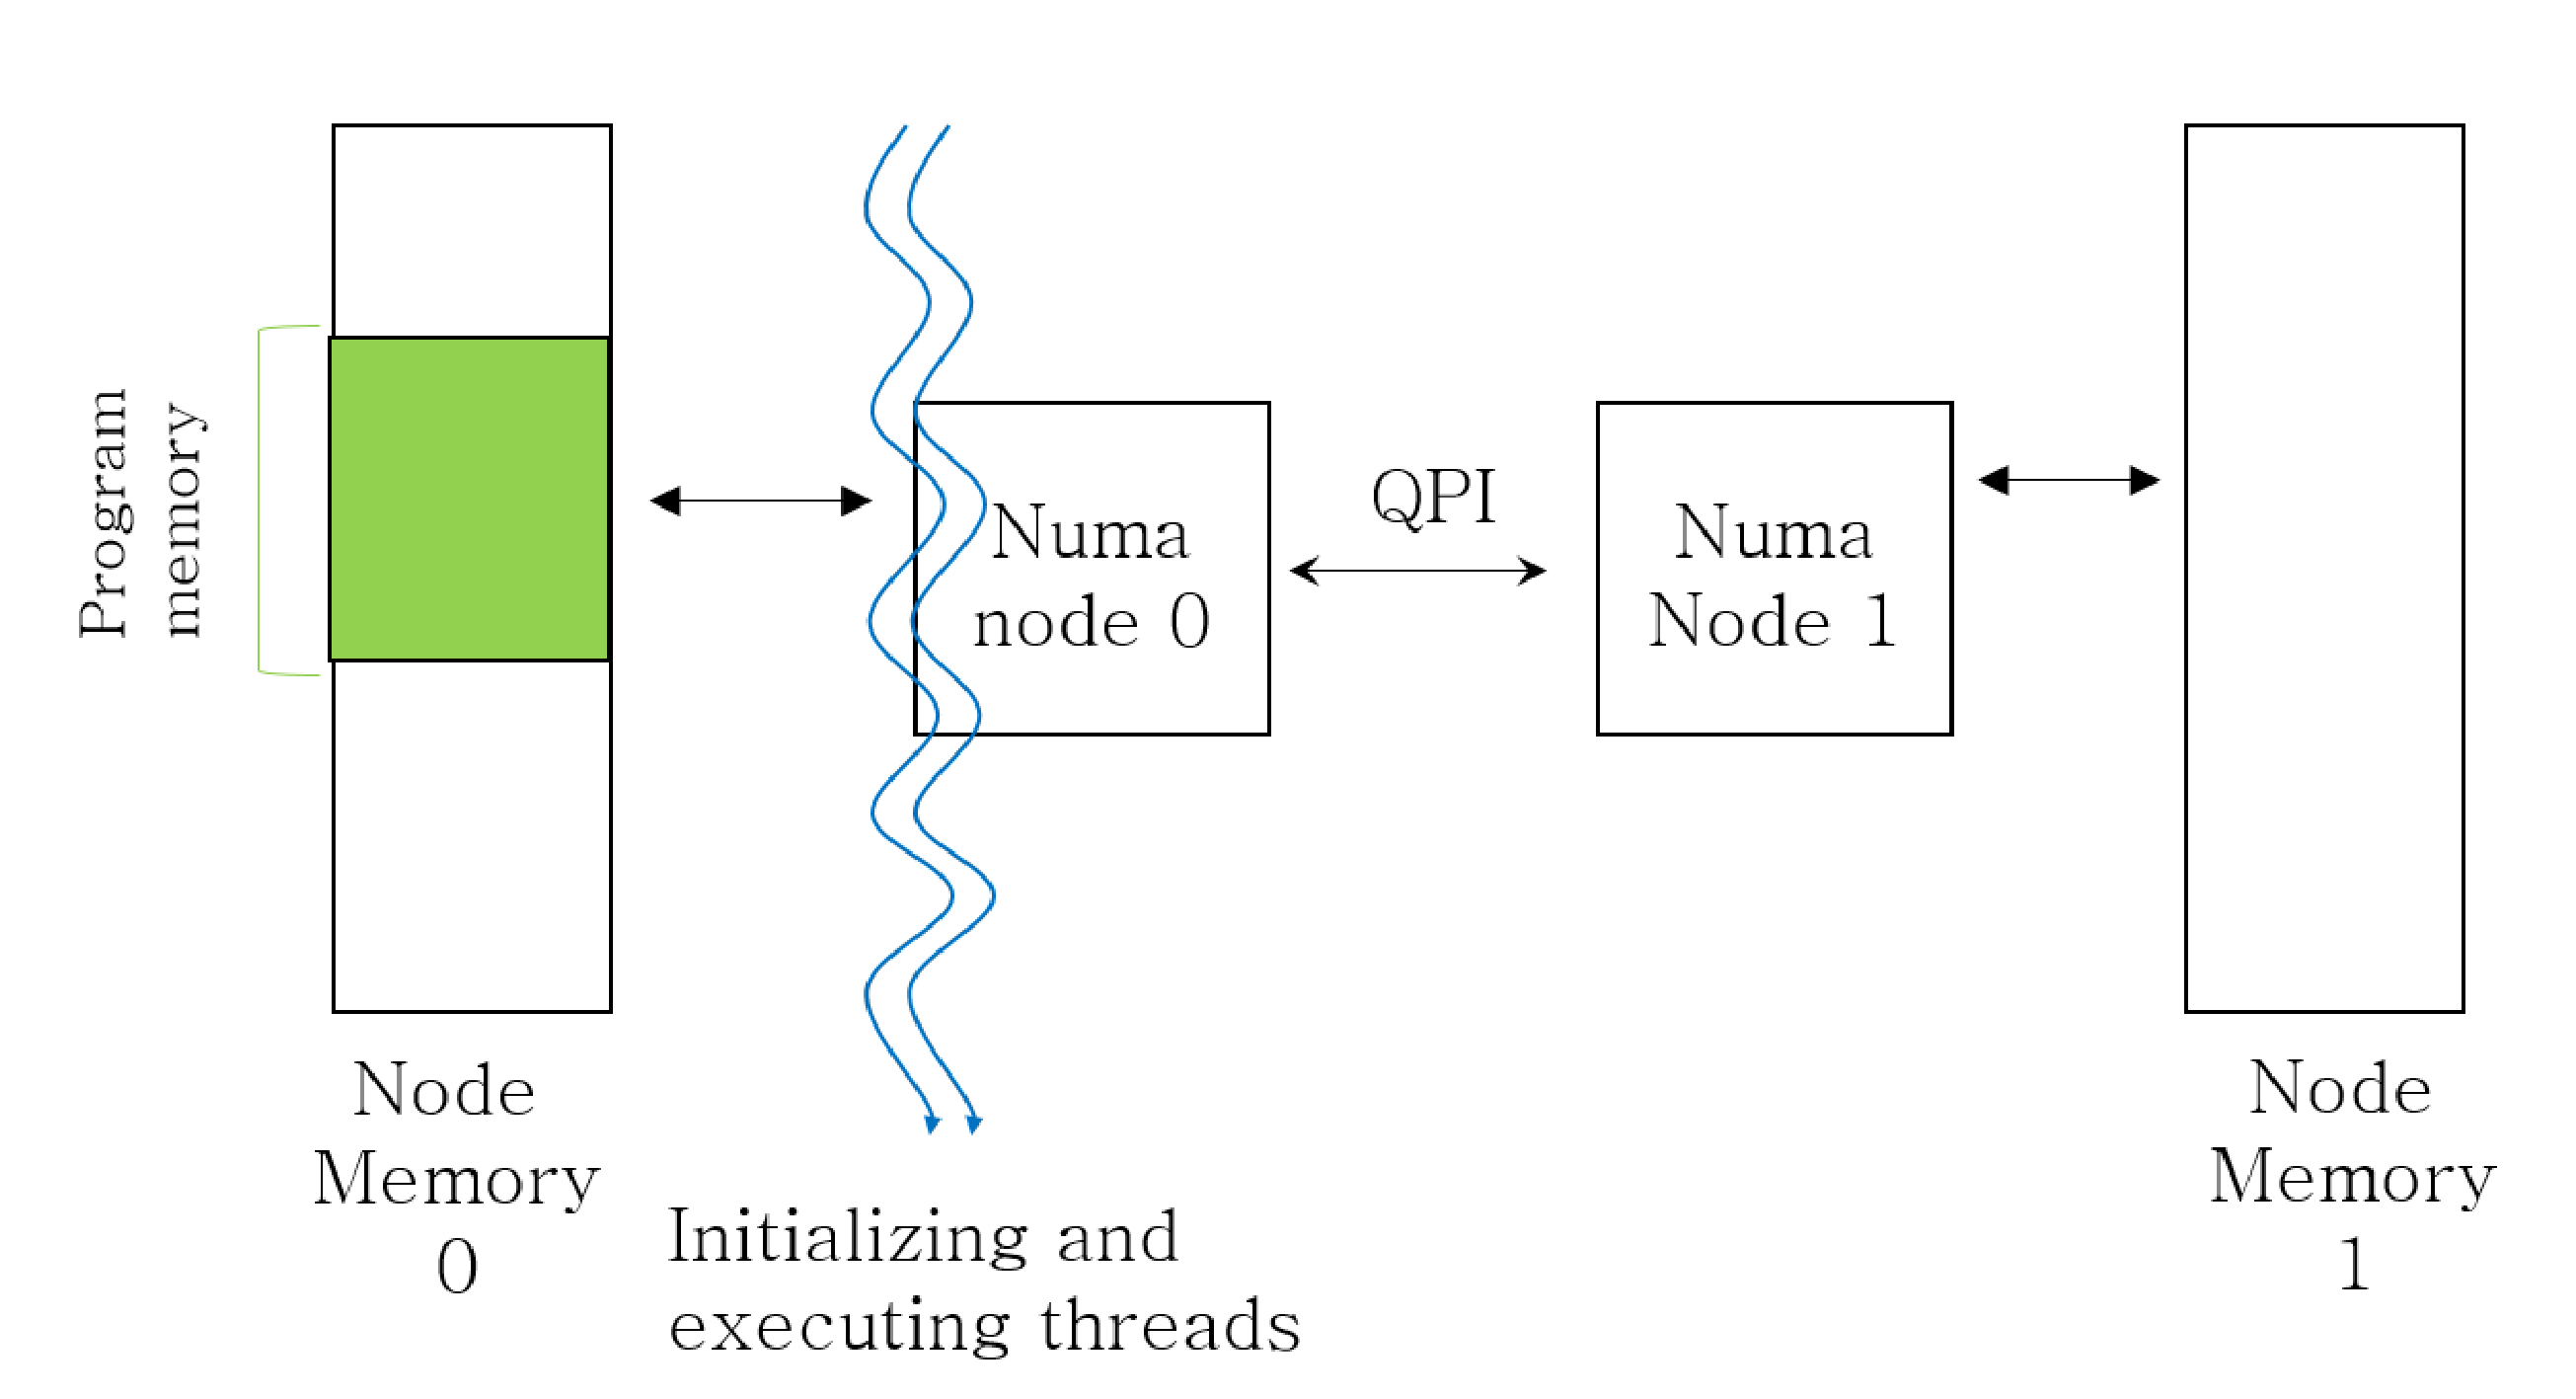
\includegraphics[width=.8\textwidth]{figures/distgentt-local.eps}
		\caption[Depiction of the working of the distgen vanilla local scenario with two threads]{Depiction of the distgen vanilla local with two running threads. Both threads are in the same NUMA node, therefore only local accesses will be performed.}
		\label{fig:dgentt-local}
\end{figure}

\begin{figure}[th]
	\centering
		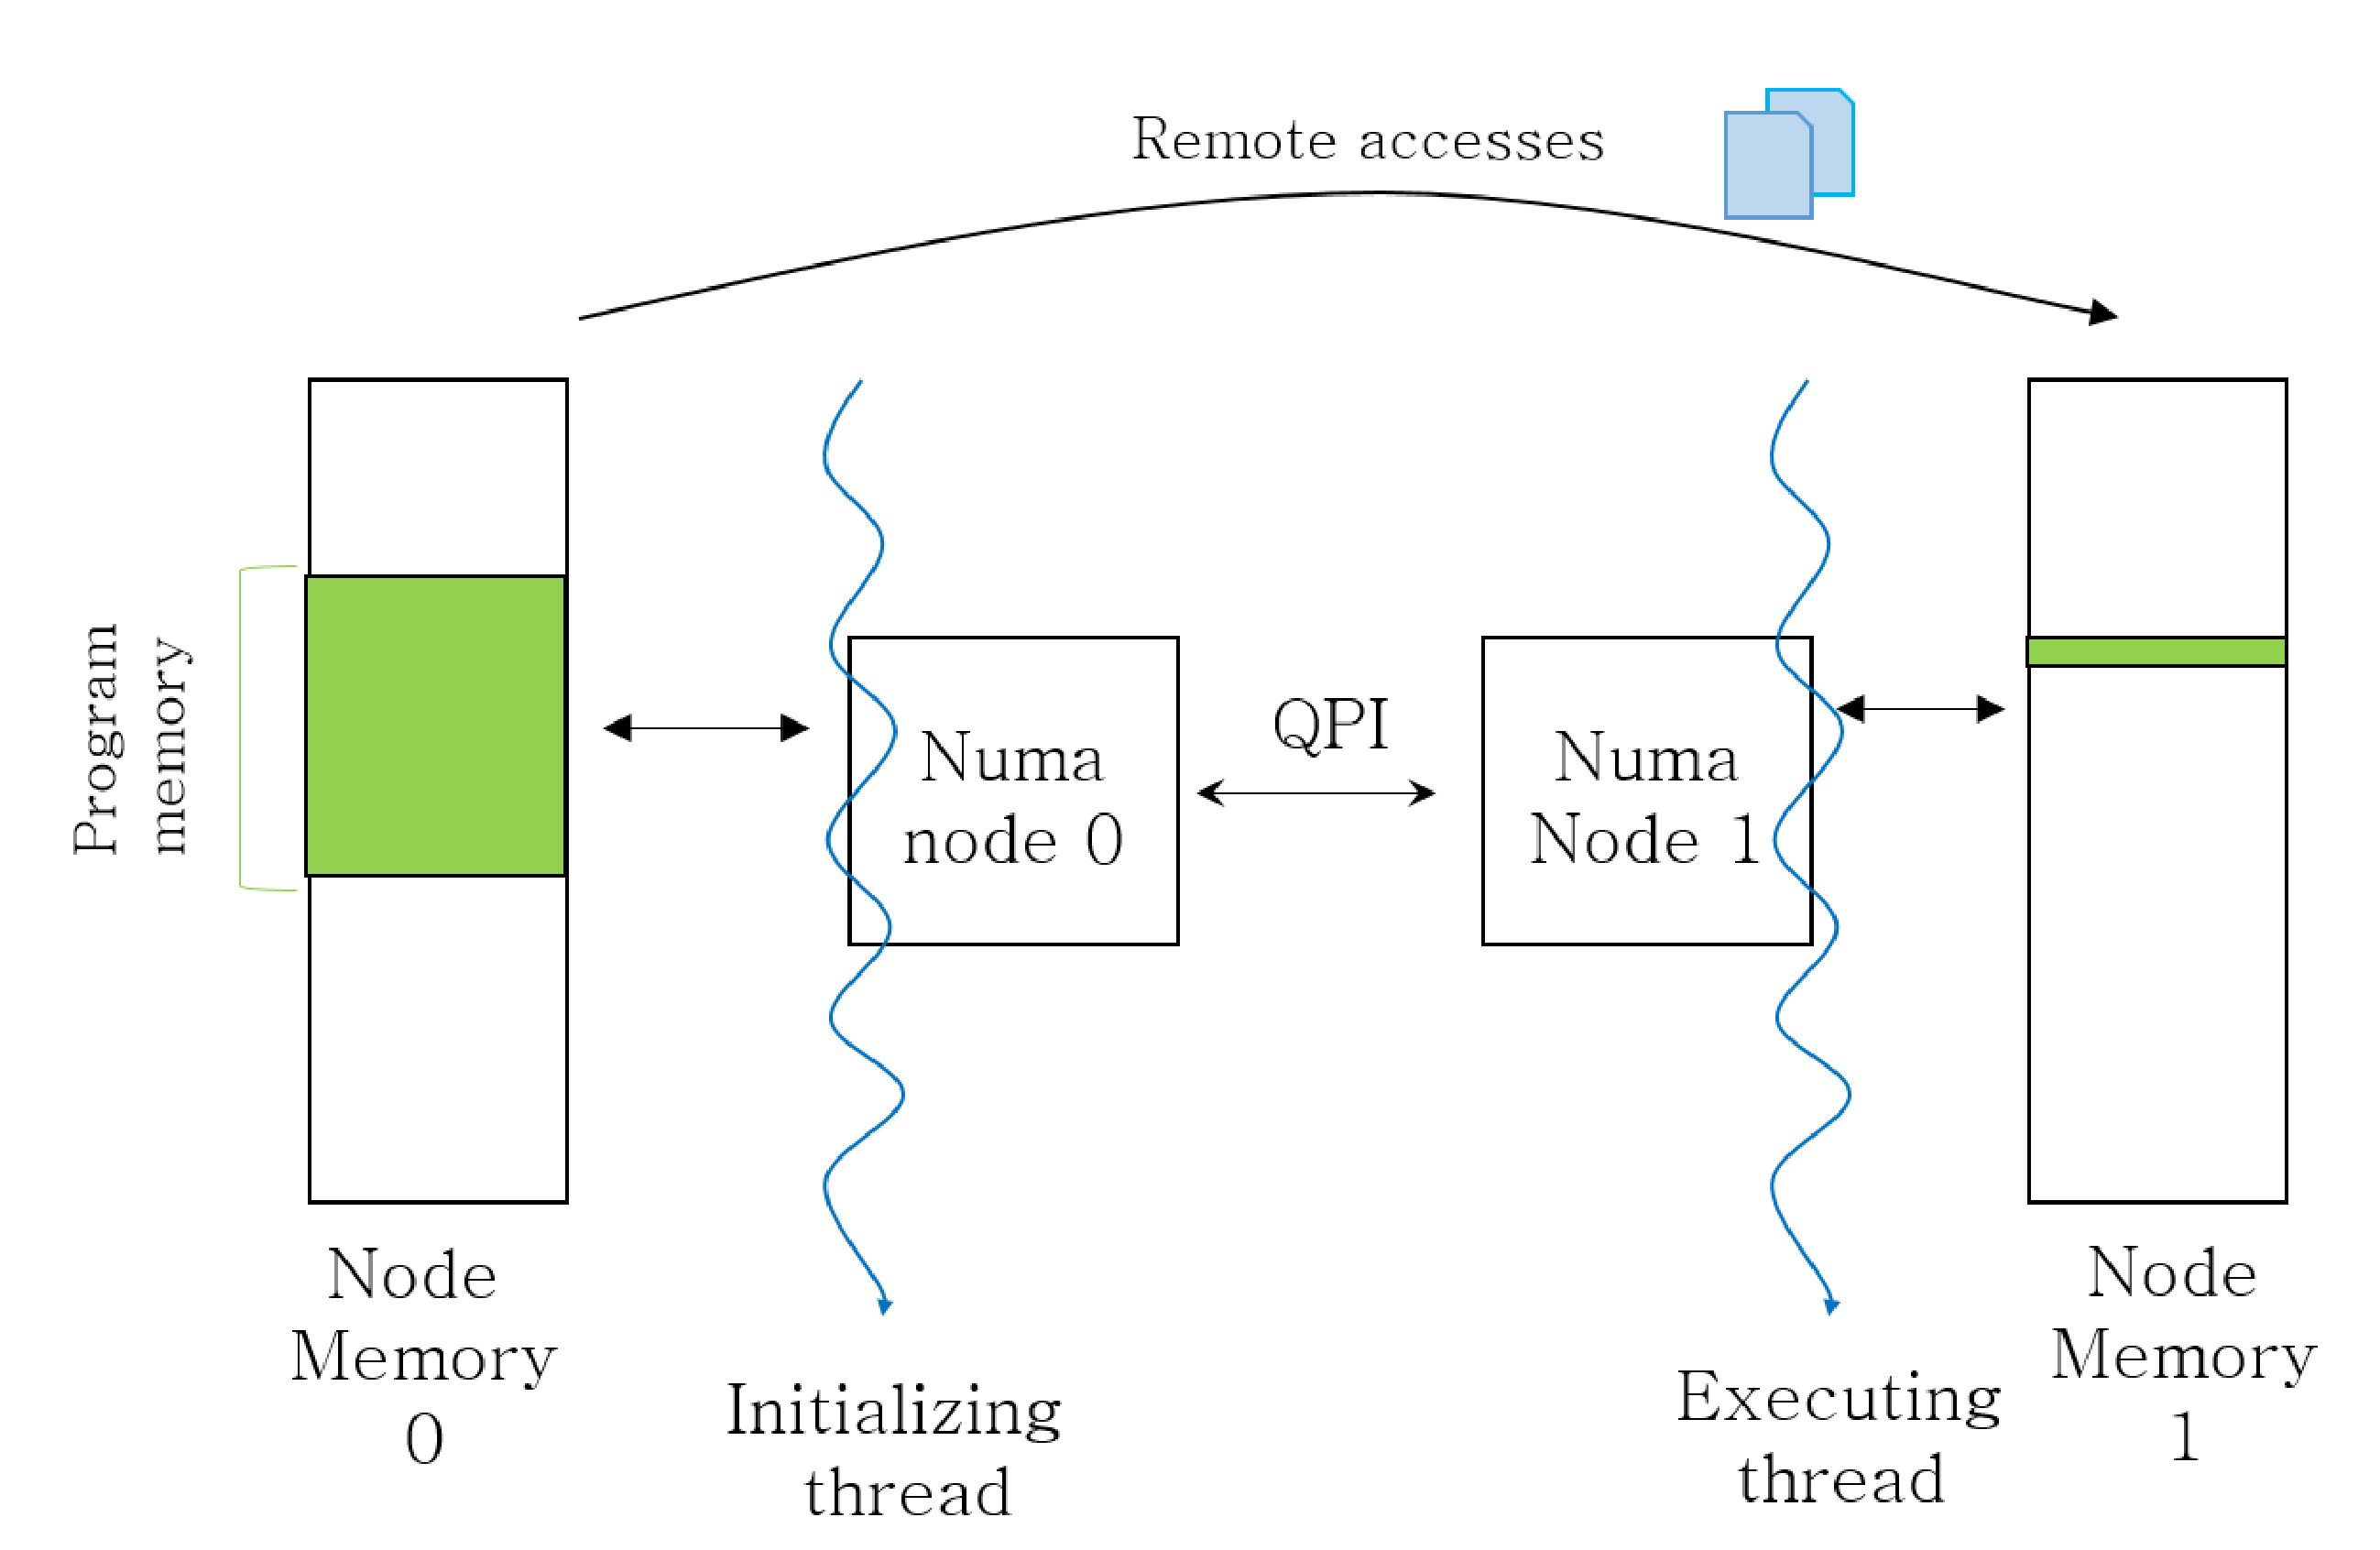
\includegraphics[width=.8\textwidth]{figures/distgentt-remote.eps}
		\caption[Depiction of the working of the distgen vanilla remote scenario with two threads]{Depiction of the distgen vanilla remote with two running threads. Each thread is pinned to a different NUMA node, which causes a lot of remote accesses to be done by the running thread.}
		\label{fig:dgentt-remote}
\end{figure}

\begin{itemize}
	\item The \textbf{vanilla local scenario} is the code in its original form, two threads are run in the same NUMA node.
	\item The \textbf{vanilla remote scenario}: Each thread runs on a separate NUMA node. The first thread initializes the memory space and the second thread accesses it. 
	\item The \textbf{SPM scenario} is the same as the vanilla remote scenario but this time the program execution will be overseen by the SPM tool and the pages observed to be accessed more from a remote node are moved to the node that originates the greater number of memory accesses.
	\item The \textbf{moveall} scenario is a distgen modification based on vanilla remote that after a determinate time of execution will move all the memory pages from a remote node to a local node.
\end{itemize}

Every one of this scenarios has a specific significance for the measurement of the performance: The vanilla local scenario shows the maximum speed possible for the given algorithm, Vanilla remote will show how much performance deteriorates when the algorithm is forced to perform many remote accesses in order to fetch the required data, moveall is a reference scenario that tells how much it is possible to fix the performance degradation by taking the pages placed in a remote node and bringing them close to the executing node and SPM also tries to fix the slowdown caused by the remote placement of the pages, but since the SPM does not know about the internal implementation of the supervised process, it will only move the pages that the PMU reports as remote accesses. The closer SPM's results are to the moveall scenario, the best performing the SPM tool is. Figures \ref{fig:dgentt-local} and \ref{fig:dgentt-remote} present depictions of both local and remote vanilla scenarios.

In order to be able to be able to place the pages remotely a modification has to be made to the original distgen code where the initialization is done by the master thread and the access is done only by the other thread, which is not the master. To determine whether the two threads are placed in a local node the environment variable \textit{GOMP\_CPU\_AFFINITY} is manipulated in order to determine the core in which the running threads will be placed. The availability of this modified two threads version is described in code listing 5 in Appendix \ref{app:coderes}.


\subsubsection{Performance for the random mode}\label{subsection:res-dgrandom-2t-scens}

Tables Tabelle 1 and Tabelle 2 Show the results of the execution of distgen random. Figures Abbildung 7: Normalized execution times for distgen random with two threads Abbildung 7 and Abbildung 8 show the execution times and throughputs respectively as a normalized quantity in respect to the distgen vanilla result which means that a value closer to 1 resembles a performance closer to that obtained in the local algorithm. For this random version of the distgen did a very good job with a performance very similar to the moveall situation, which is the theorethical maximum that can be archived. Another important result that appears in most of the measurements is that the performance of the moveall strategy after moving the pages never gets to be the same as that obtained in the local version, effect that has to be researched further.
As for the performance of the SPM it can be seen from Tabelle 3 the percentage of caught pages remain above 40 percent with decreasing value as the domain gets bigger. This happens because with a bigger domain size the observation time occupies a smaller relative portion of the total execution time and therefore less samples can be caught.


\begin{table}
	\centering
		\begin{tabularx}{\textwidth}{|l|l|l|l|X|}
		\hline
			Size & Vanilla local & Vanilla Remote & Moveall after 45s & SPM \\
			\hline
			400G & 61.470 & 102.573 & 85.375 & 80.221\\
			\hline
			600G & 91.382 & 154.340 & 124.067 & 134.695\\
			\hline
			800G & 125.757 & 215.269 & 200.078 & 187.817\\
			\hline
			1T & 151.291 & 151.291 & 198.249 & 202.729\\
			\hline
		\end{tabularx}
		\caption{Execution time given in seconds of the different distgen scenarios in random mode.}
		\label{table:res-tbl-dgentimrdm2t}
\end{table}

\begin{table}
	\centering
		\begin{tabularx}{\textwidth}{|l|l|l|l|X|}
		\hline
			Size & Vanilla local & Vanilla Remote & Moveall after 45s & SPM \\
			\hline
			400G & 1.12973E+08 & 6.77034E+07 & 1.00708E+08 & 9.68249E+07\\
			\hline
			600G & 1.13992E+08 & 6.74924E+07 & 8.24585E+07 & 9.35968E+07\\
			\hline
			800G & 1.10442E+08 & 6.45197E+07 & 7.36434E+07 & 7.10097E+07\\
			\hline
			1T & 1.14753E+08 & 6.66698E+07 & 8.85143E+07 & 9.39763E+07\\
			\hline
		\end{tabularx}
		\caption{Execution throughput given in reads per second of the different distgen scenarios in random mode.}
		\label{table:res-tbl-dgentrgrdm2t}
\end{table}

\begin{table}
	\centering
		\begin{tabularx}{\textwidth}{|l|l|l|}
		\hline
			Size & Moved pages & Moved pages \%  \\
			\hline
			400G & 422971 & 108.280576 \\
			\hline
			600G & 372289 & 63.53732267 \\
			\hline
			800G & 413297 & 52.902016 \\
			\hline
			1T & 423478 & 43.3641472 \\
			\hline
		\end{tabularx}
		\caption{Number of pages moved in the SPM scenario}
		\label{table:res-tbl-dgenmvdrdm2t}
\end{table}


\begin{figure}[th]
	\centering
		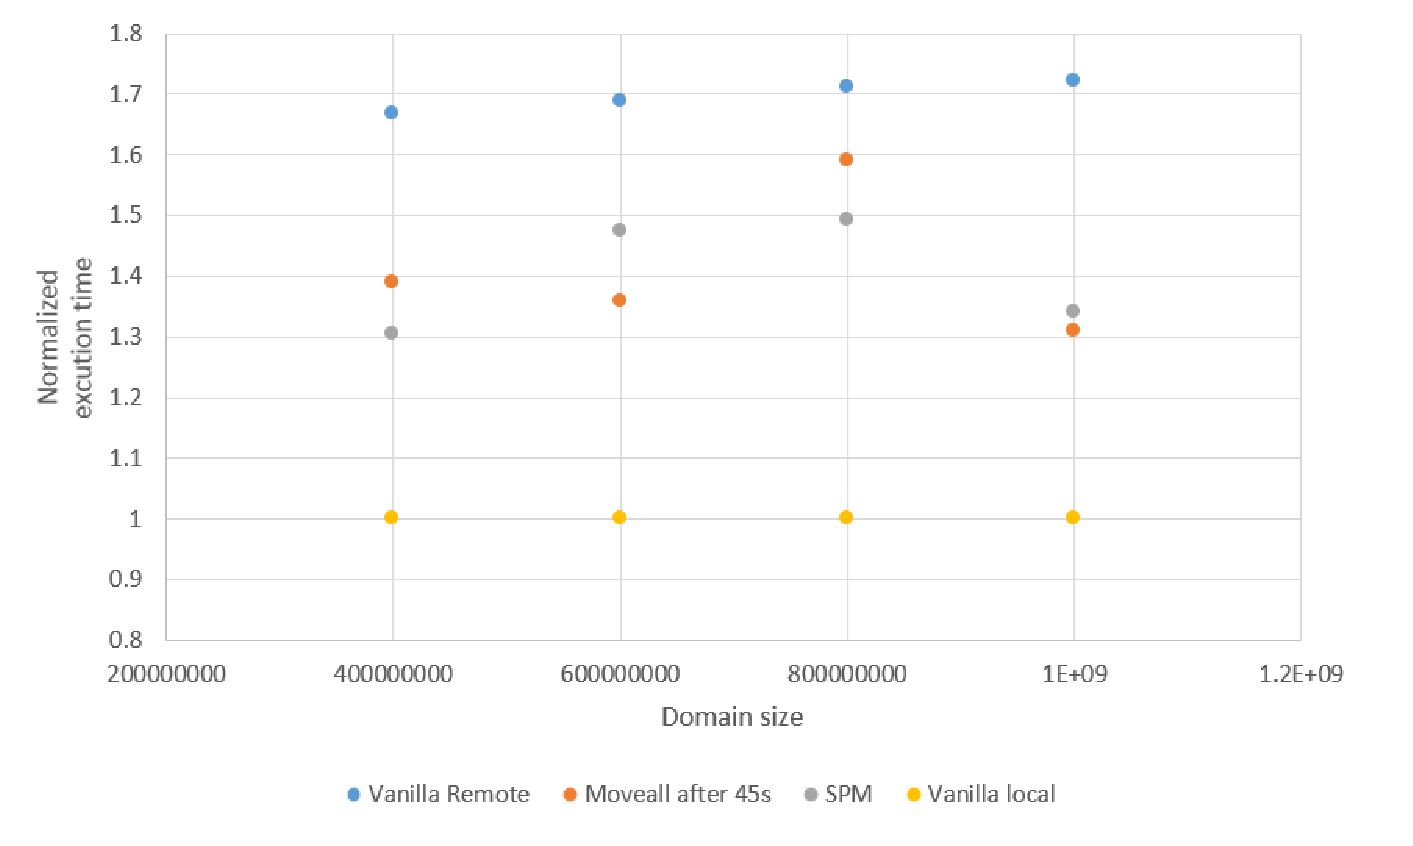
\includegraphics[width=.8\textwidth]{figures/time-dgentt-random.eps}
		\caption{Normalized execution times for distgen random with two threads}
		\label{fig:res-time-dgentt-ser}
\end{figure}

\begin{figure}[th]
	\centering
		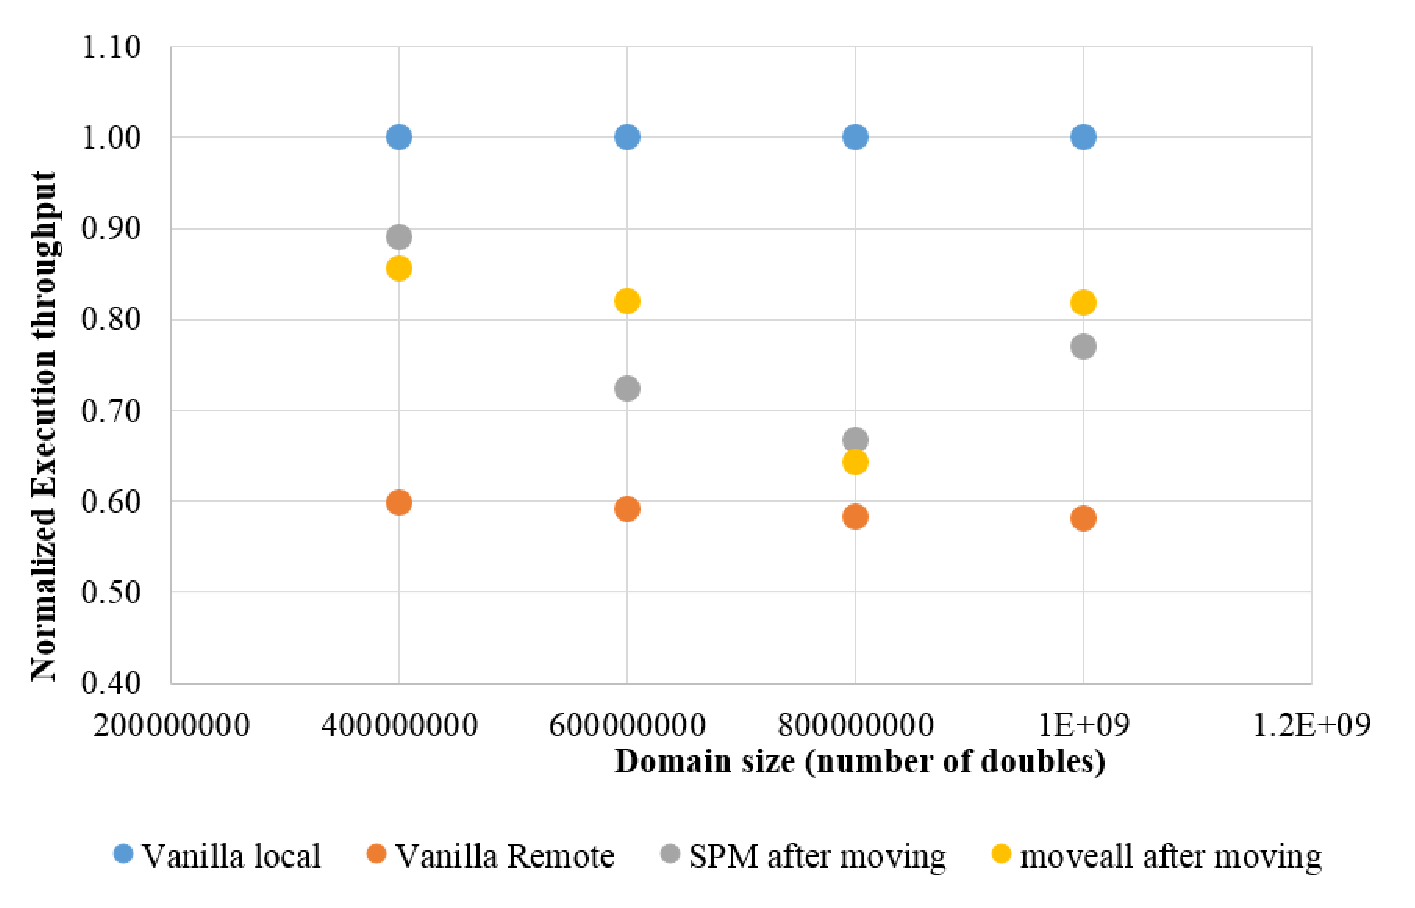
\includegraphics[width=.8\textwidth]{figures/thrput-dgentt-randm.eps}
		\caption{Normalized execution throughput for distgen random with two threads}
		\label{fig:thrput-dgentt-randm}
\end{figure}

\subsubsection{Performance for the sequential mode}\label{subsection:res-dgseq-2t}
In this opportunity the serial version of distgen is run. Because of the faster running time of this algorithm, the number of iterations is doubled to 2000 to obtain a long enough execution time.  Tabelle 4 and Tabelle 5 show the execution time and performance results and the Abbildung 9 and Abbildung 10 show the normalized values with respect to distgen vanilla. In comparison to the serial version the performance of the SPM tool is not as good and only matches that of the moveall scenario in with the smallest size. Part of this slowdown can be blamed on the smaller portion of pages that the tool is getting.

\begin{table}[th]
	\centering
		\begin{tabularx}{\textwidth}{|l|l|l|l|X|}
		\hline
			Size & Vanilla local & Vanilla Remote & Moveall after 45s & SPM \\
			\hline
			400G & 55.924 & 92.534 & 75.146 & 75.969\\
			\hline
			600G & 83.894 & 138.851 & 104.407 & 117.433\\
			\hline
			800G & 111.823 & 185.144 & 133.699 & 159.905\\
			\hline
			1T & 139.810 & 231.453 & 163.018 & 199.576\\
			\hline
		\end{tabularx}
		\caption{Execution time for the different scenarios of the distgen sequential algorithm with units given in seconds.}
		\label{table:table:res-tbl-dgenmvdseq2t}
\end{table}

\begin{table}[th]
	\centering
		\begin{tabularx}{\textwidth}{|l|l|l|l|X|}
		\hline
			Size & Vanilla local & Vanilla Remote & Moveall after 45s & SPM \\
			\hline
			SZ1 & 2.48368E+08 & 1.50106E+08 & 2.37768E+08 & 2.37636E+08\\
			\hline
			SZ2 & 2.48350E+08 & 1.50048E+08 & 1.96037E+08 & 2.37708E+08\\
			\hline
			SZ3 & 2.48409E+08 & 1.50039E+08 & 1.86950E+08 & 1.48624E+08\\
			\hline
			SZ3 & 2.48352E+08 & 1.50023E+08 & 1.48624E+08 & 2.37542E+08\\
			\hline
		\end{tabularx}
		\caption{Execution throughput for the different scenarios of the distgen sequential algorithm with units given in reads per second.}
		\label{table:table:res-tbl-dgentimseq2t}
\end{table}

\begin{table}[th]
	\centering
		\begin{tabularx}{\textwidth}{|l|l|X|}
		\hline
			Size & Moved pages & Moved pages \%  \\
			\hline
			400G & 232777 & 59.590912 \\
			\hline
			600G & 234551 & 40.03003733\\
			\hline
			800G & 226748 & 29.023744 \\
			\hline
			1T & 233191 & 23.8787584 \\
			\hline
		\end{tabularx}
		\caption{Number of pages moved in the distgen sequential scenario.}
		\label{table:res-tbl-dgenmvdseq2t}
\end{table}

\begin{figure}[th]
	\centering
		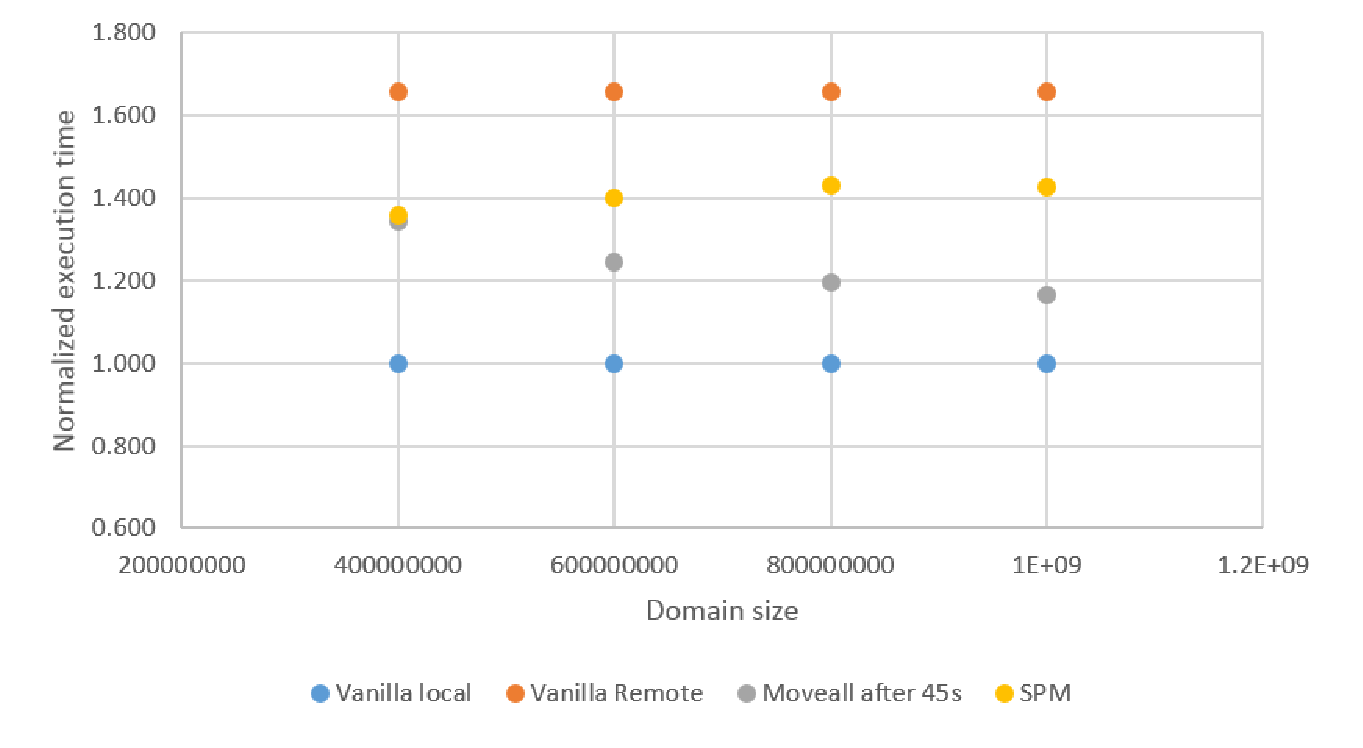
\includegraphics[width=.8\textwidth]{figures/time-dgentt-ser.eps}
		\caption{Normalized execution speed for the different scenarios of the distgen sequential with two threads with respect to the vanilla local scenario}
		\label{fig:time-dgentt-ser}
\end{figure}

\begin{figure}[th]
	\centering
		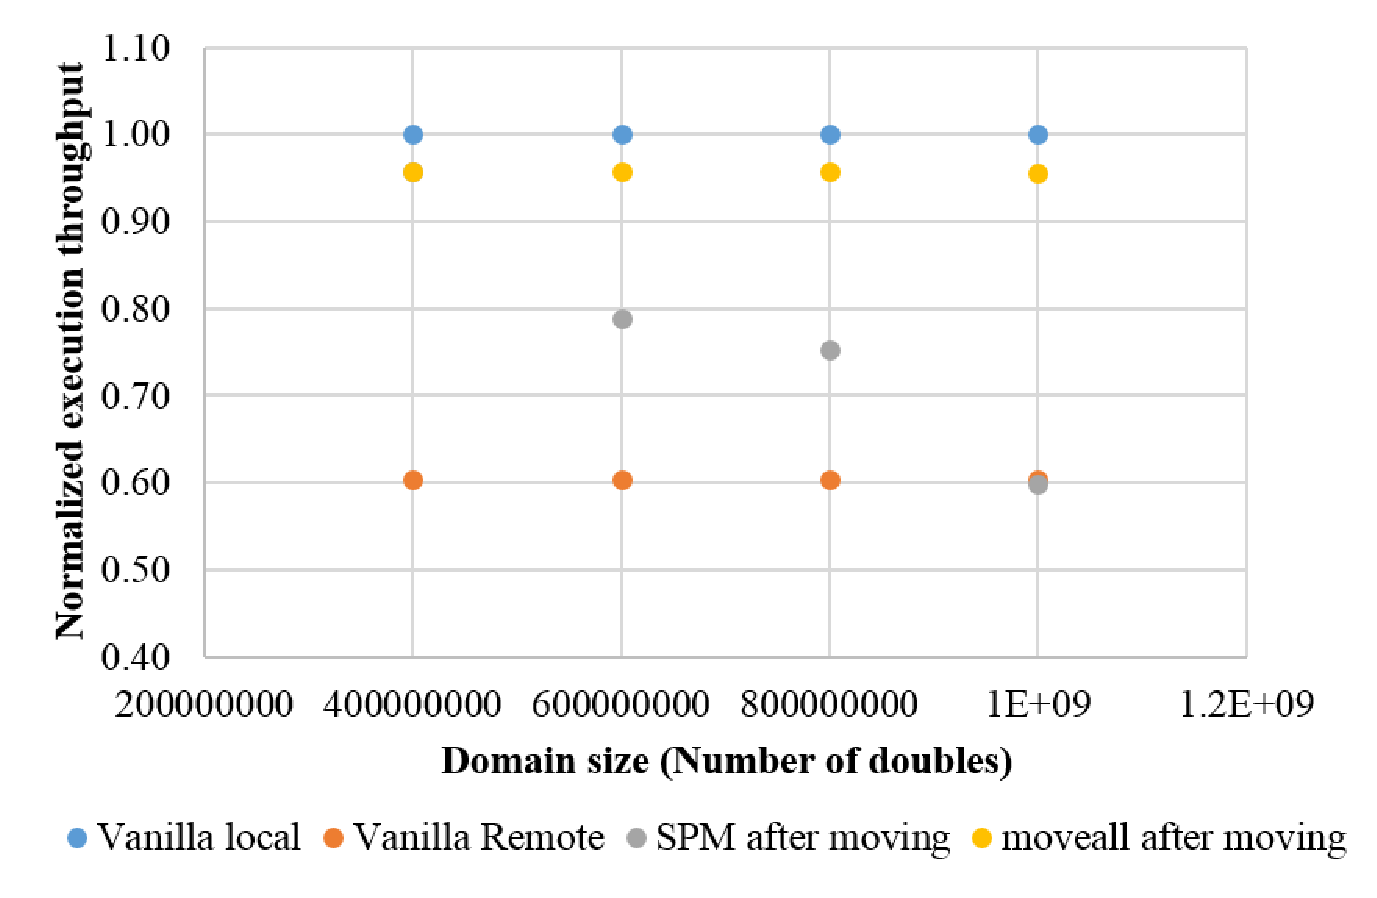
\includegraphics[width=.8\textwidth]{figures/thrput-dgentt-ser.eps}
		\caption{Normalized execution throughput for the different scenarios of the distgen sequential with two threads with respect to the vanilla local scenario.}
		\label{fig:thrput-dgentt-ser}
\end{figure}

\subsection{SPM and distgen with all threads employed}\label{subsection:res-spmydistgen-at}

The scenarios used here follow the same logic as what was shown in the previous section, but now we want to go further and try a contention scenario where more cores are running the algorithm. For this test all the cores except two were used, the two saved are used for running SPM. In the remote cases, every core is mapped to an opposite core in the opposed numa node and the data will be allocated in this remote node.

\subsubsection{Performance for the random mode}\label{subsection:time-dgenat-random.eps}


\begin{table}[th]
	\centering
		\begin{tabularx}{\textwidth}{|l|l|l|l|X|}
		\hline
			Size & Vanilla local & Vanilla Remote & Moveall after 45s & SPM \\
			\hline
			90G & 83.51 & 196.688 & 152.959 & 155.405\\
			\hline
			110G & 103.617 & 242.471 & 184.673 & 191.259\\
			\hline
			130G & 129.617 & 282.619 &194.029 & 210.215\\
			\hline
			150G & 141.588 & 329.403 & 260.219 & 254.283\\
			\hline
		\end{tabularx}
		\caption{Completion time in seconds for the random distgen with 30 threads employed}
		\label{table:res-dgenrdmat-time}
\end{table}

\begin{figure}[th]
	\centering
		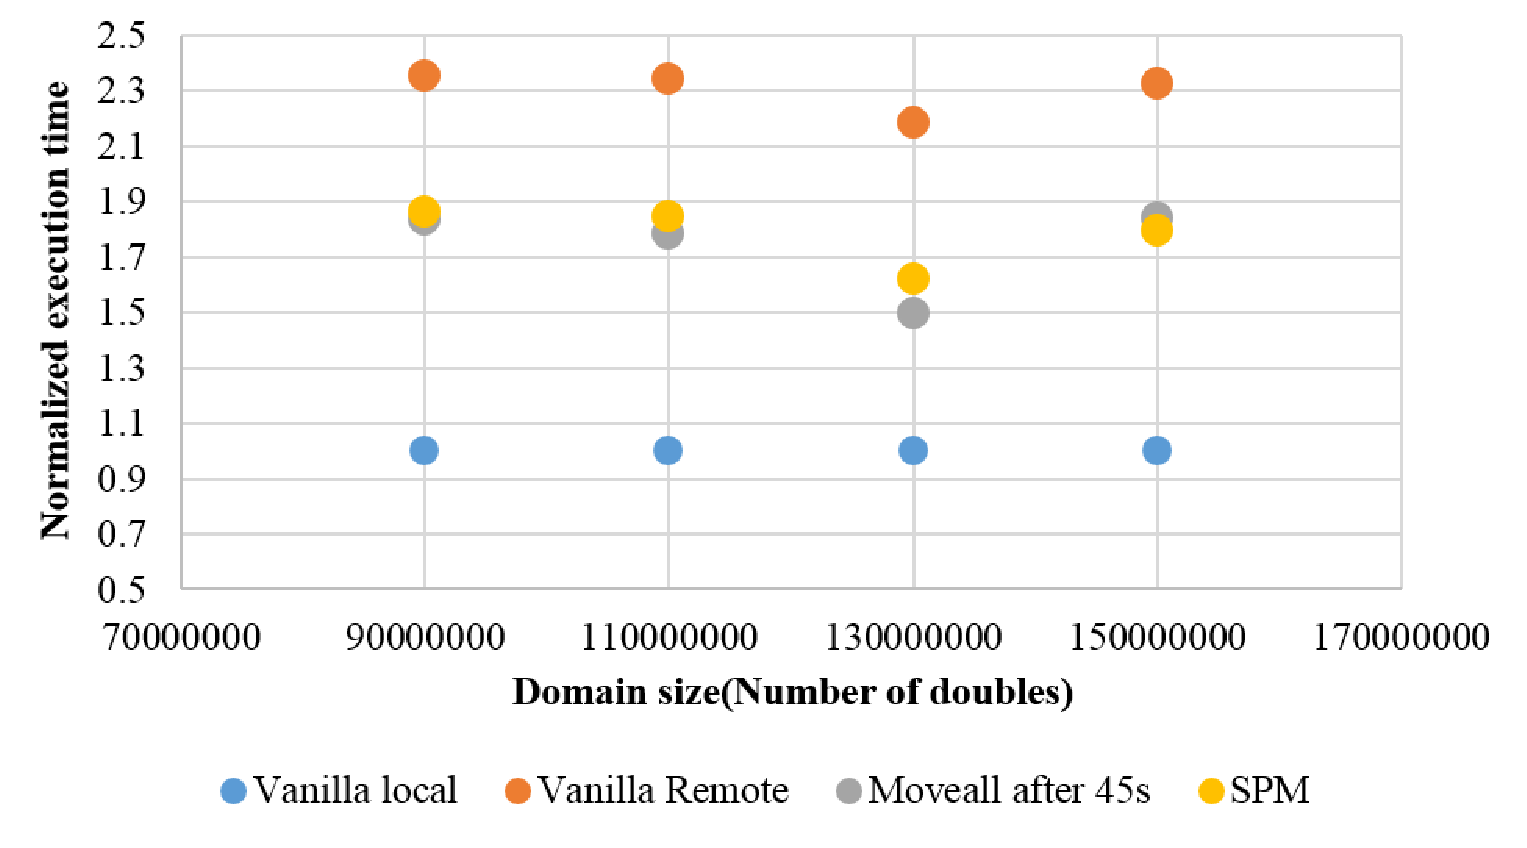
\includegraphics[width=.8\textwidth]{figures/time-dgenat-random.eps}
		\caption{Normalized execution time for the random distgen cases with 30 threads employed.}
		\label{fig:time-dgenatt-ran}
\end{figure}

\subsubsection{Performance for the sequential mode}\label{subsection:time-dgenat-seq.eps}

\begin{table}[th]
	\centering
		\begin{tabularx}{\textwidth}{|l|l|l|l|X|}
		\hline
			Size & Vanilla local & Vanilla Remote & Moveall after 45s & SPM \\
			\hline
			90G & 127.763 & 341.35 & 152.959 & 262.535\\
			\hline
			110G & 156.145 & 417.683 & 184.673 & 331.794\\
			\hline
			130G & 184.482 & 493.134 & 194.029 & 395.134\\
			\hline
			150G & 212.992 & 569.438 & 260.219 & 465.617\\
			\hline
		\end{tabularx}
		\caption{Latencies and timing table}
		\label{table:res-dgenrdmat-movpg}
\end{table}

\begin{table}[th]
	\centering
		\begin{tabularx}{\textwidth}{|c|c|c}
		\hline
			Size & Moved pages & Moved pages \%  \\
			\hline
			90G & 4438270 & 84.16274963 \\
			\hline
			110G & 4556914 & 54.38554704 \\
			\hline
			130G & 3526065 & 46.29090462 \\
			\hline
			150 & 4647763 & 52.88121458 \\
			\hline
		\end{tabularx}
		\caption{Number of moved pages by the SPM tool for the distgen random case with all threads engaged}
		\label{table:res-tbl-dgenmvdseqat}
\end{table}

\begin{table}[th]
	\centering
		\begin{tabularx}{\textwidth}{|l|l|X|}
		\hline
			Size & Moved pages & Moved pages \%  \\
			\hline
			90G & 770653 & 13.70049778 \\
			\hline
			110G & 809007 & 11.76737455 \\
			\hline
			130G & 809901 & 9.96801230 \\
			\hline
			150 & 853033 & 9.099018667 \\
			\hline
		\end{tabularx}
		\caption{Number of moved pages by the SPM tool for the distgen random case with all threads engaged.}
		\label{table:res-tbl-dgenmvdseqat}
\end{table}

\begin{figure}[th]
	\centering
		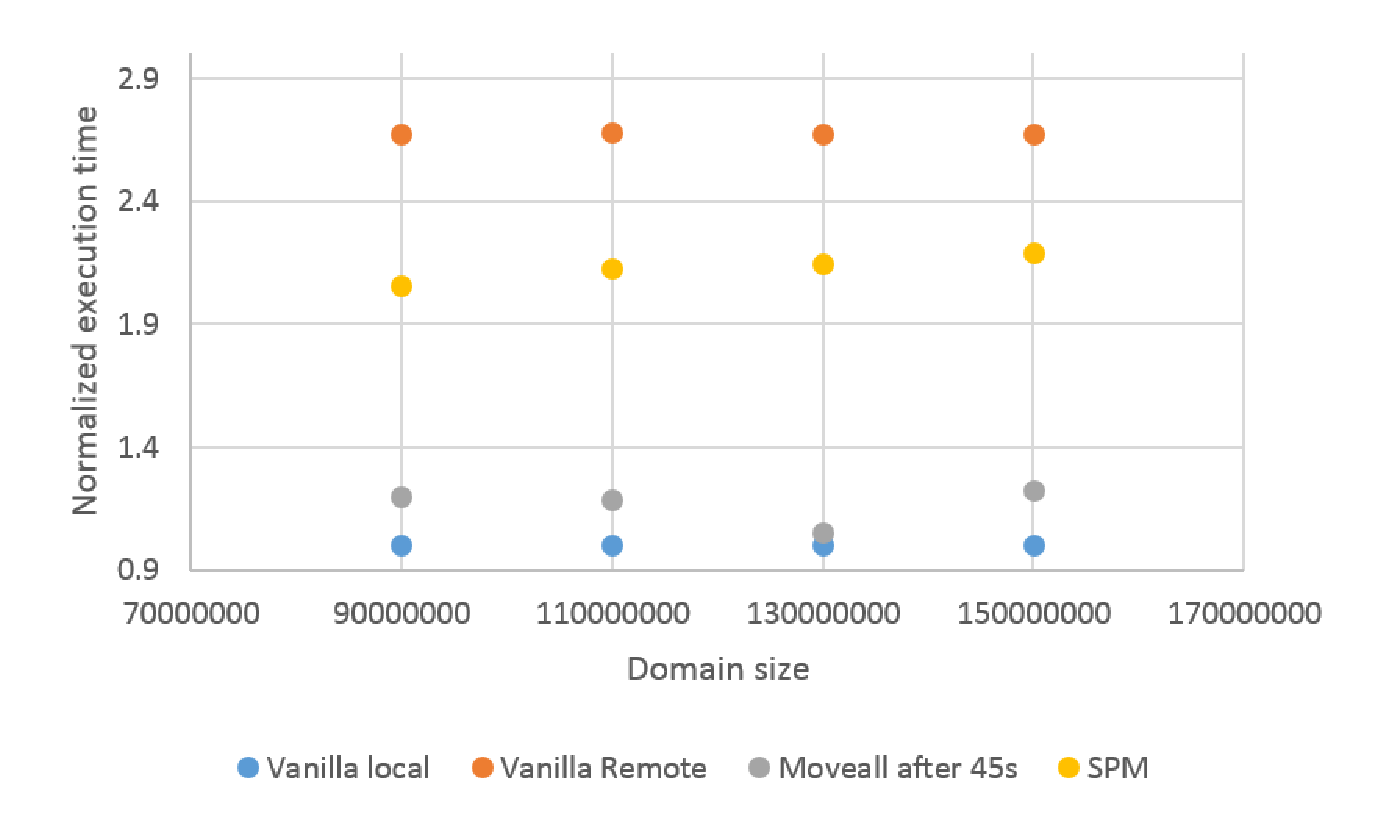
\includegraphics[width=.8\textwidth]{figures/time-dgenatt-ser.eps}
		\caption{Normalized execution time for the sequential distgen cases with 30 threads employed.}
		\label{fig:time-dgenatt-ser}
\end{figure}

\subsubsection{Measuring the effect of SPM's action}\label{subsection:time-dgenat-action.eps}

\begin{figure}[th]
	\centering
		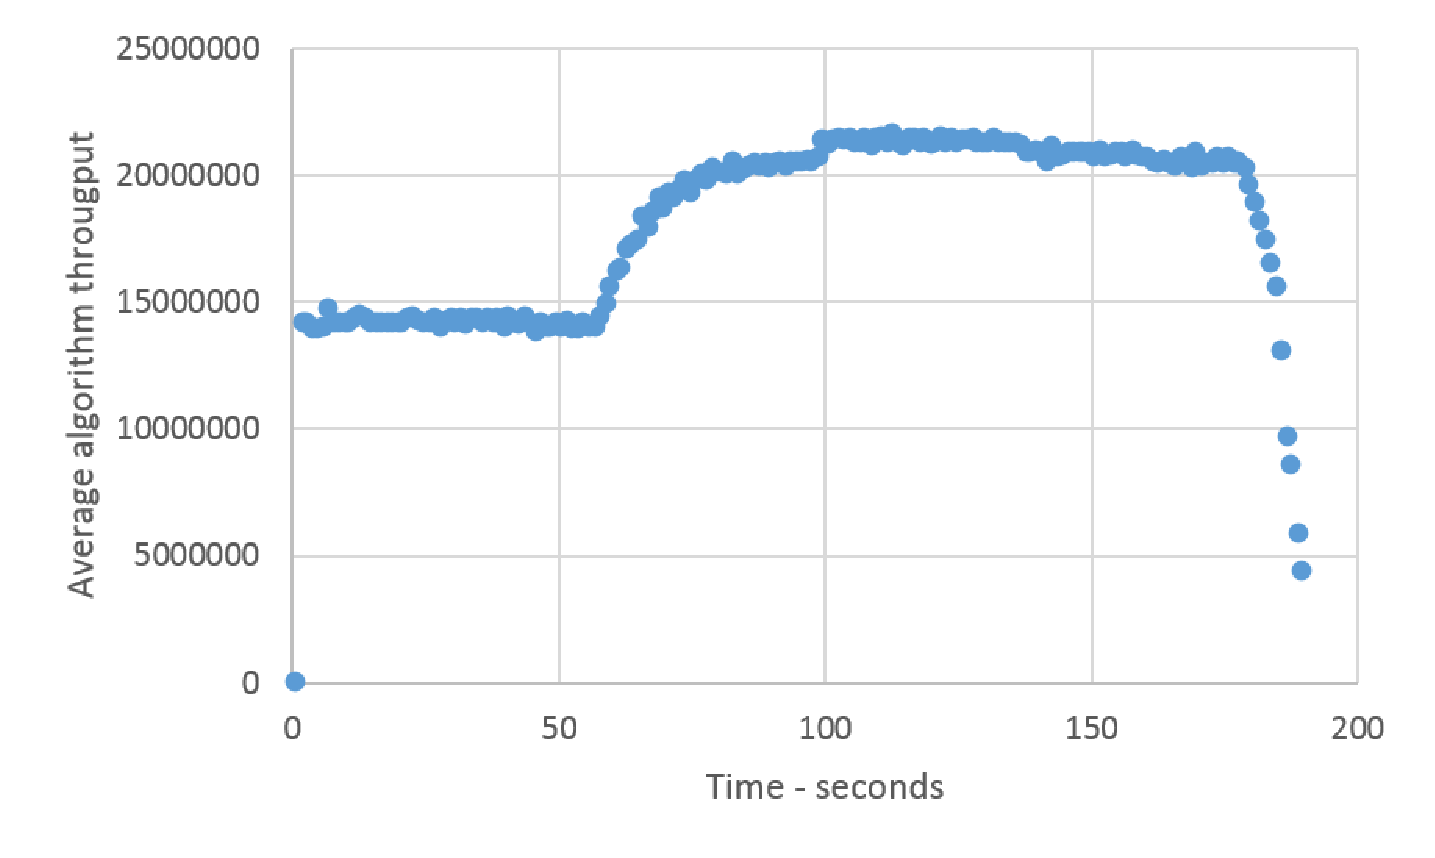
\includegraphics[width=.8\textwidth]{figures/at-thrput-random.eps}
		\caption{View of the average throughput during the execution of distgen under SPM supervision. The page migration is done at time 45.}
		\label{fig:at-spmactn-thgput}
\end{figure}

\begin{figure}[th]
	\centering
		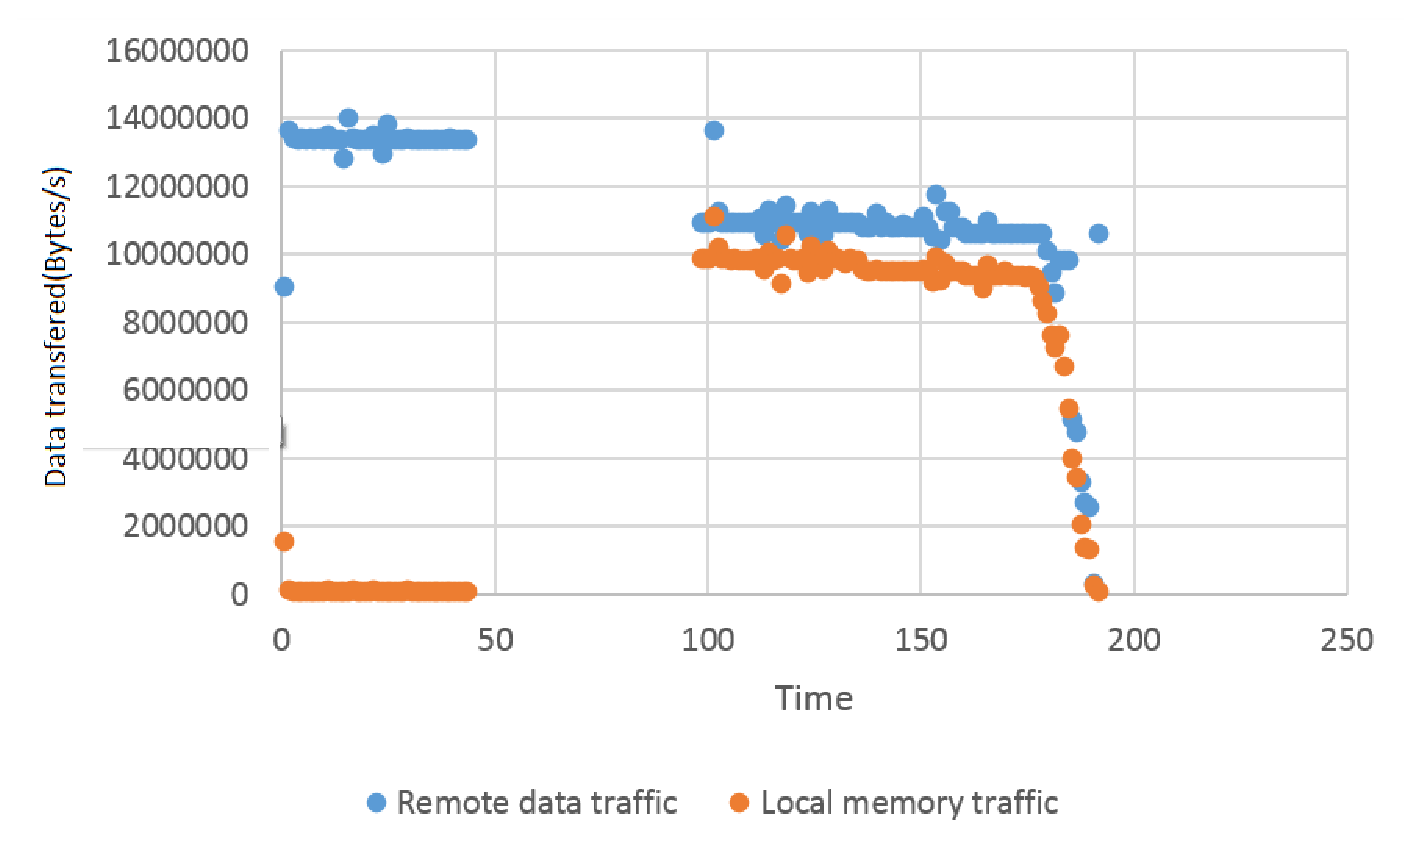
\includegraphics[width=.8\textwidth]{figures/at-transfer-random.eps}
		\caption{View of the average and local and remote transfer rates during the execution of distgen under SPM supervision. The page migration is done at time 45.}
		\label{fig:at-spmactn-trsfer}
\end{figure}